% A workaround to allow relative paths in included subfiles
% that are to be compiled separately
% See https://tex.stackexchange.com/questions/153312/subfiles-inside-a-subfile-using-relative-paths
\providecommand{\main}{..}
\documentclass[\main/thesis.tex]{subfiles}

\begin{document}

\chapter{Evaluation}
\label{cha:evaluation}
This chapter presents an evaluation of the implementation developed in \rcha{method}.
The results presented also represent one of the first evaluations of \gls{power10}'s \gls{mma} facility.
Given that the evaluation was performed on test~\bk{There's a better word for this, I'm sure.} hardware, the results are expected to be representative of the hardware that will eventually be available to consumers but not exactly the same.
This could be due to anything from frequency changes to firmware changes or actual silicon changes.

\section{Experimental Setup}
This section presents details on resources used and processes performed to produce the results in \rsec{caveats} and onwards.

\subsection{Machine Details}
Experiments were conducted on a \gls{power10} machine provided by \gls{ibm}.
The processor is not yet available to the public but relevant details are presented in \rtab{machineInfo}.
The listed core counts are per socket while the thread counts are per core.
The machine runs Linux with a 64-bit kernel at version 5.10.0-17496-g41bc5268c5e8.

\begin{table}[t]
  \centering
  \begin{tabular}{c | c}
    & IBM POWER10\\\hline
    Cores/Threads & 15/8\\
    L1i cache & 720KiB\\
    L1d cache & 480KiB\\
    Frequency & 3.65 GHz\\
  \end{tabular}
  \caption{POWER10 machine info.}
  \label{tab:machineInfo}
\end{table}

\subsection{Compilation}
All binaries are compiled with Clang version 13.0.0\footnotemark at the highest optimisation level (\code{-O3}) and are tuned to the processor (\code{-mcpu=pwr10}).
\footnotetext{At time of writing this is a development version.}
Because support for \gls{power10} was not available in mainstream \gls{llvm} when this work began, it has been implemented as part of \glslink{ibm}{IBM's} variant of \gls{llvm} which did have support.
This variant contains several platform specific, targeted optimisations focused on improving \gls{power} code; these have all been disabled so that results are representative of mainstream \gls{llvm}.

\subsection{Experimental Methodology}
\begin{figure}[t]
  \centering
  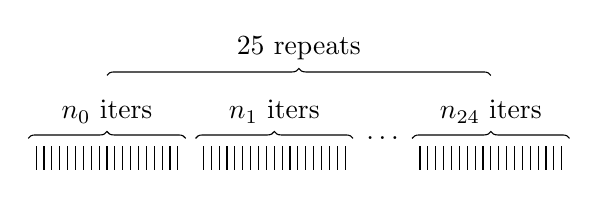
\begin{tikzpicture}[scale=1]
    \draw[decorate, decoration={brace}, align=center, shift={(0, 0)}] (0, 0) -- node[above=2] {$n_0$ iters} +(2, 0);
    \draw[decorate, decoration={brace}, align=center, shift={(2.125, 0)}] (0, 0) -- node[above=2] {$n_1$ iters} +(2, 0);
    \node[shift={(4.5, 0)}] {$\ldots$};
    \draw[decorate, decoration={brace}, align=center, shift={(4.875, 0)}] (0, 0) -- node[above=2] {$n_{24}$ iters} +(2, 0);
    \draw[decorate, decoration={brace}, align=center, shift={(1, .8)}] (0, 0) -- node[above=2] {25 repeats} +(4.875, 0);
    \foreach \x in { 0, 2.125, 4.875 }
    {
      \pgfmathsetmacro{\xStart}{\x + 0.1}
      \foreach \i in {0,...,18}
      {
        \draw[shift={(\xStart + \i * 0.1, -0.1)}] (0, 0) -- +(0, -0.3);
      }
    }
  \end{tikzpicture}
  \caption{Experiment execution process.}
  \label{fig:execution}
\end{figure}

Every measurement presented in this chapter was produced using the Google\texttrademark{} benchmark library\footnotemark~\autocite{googlebench}.
\footnotetext{At commit ab74ae5e104f72fa957c1712707a06a781a974a6.}
A sinlge measurement is the result of timing the execution of a kernel many times until statistical stability is obtained.
The framework implements a method of measuring a kernel by placing it in a loop whose exit condition is dynamically determined by the benchmark being executed.
The loop will only exit when the kernel been executed enough times.

To achieve this, a loop trip count, $n$, is determined by
\begin{enumerate*}[itemjoin={{; }}, itemjoin*={{; and }}, label=(\arabic*), after={\footnotemark.}]
  \item timing several executions of the benchmark
  \item multiplying the required time (set at one second\footnote{One second is double the default, suggested half-second time-limit.}) by $1.4$
  \item dividing by the average execution time of those executions
\end{enumerate*}
\footnotetext{This process can be verified in any upcoming table using $n \times \text{cpuTime} \approx 1.4e9$.}
The true process is more iterative and tries mulitple values in order to produce a conservative estimate for benchmarks with variation in their execution times.
For the kernels benchmarked in this chapter, which have very little variation, this is an accurate summary of the process.

\bk{Double check these numbers when they're finalised.}
While a single second may seem short, for the longest-running kernel presented (\atilde\SI{81}{\textit{\micro\second}}), this still results in roughly 17000 executions.
For the shortest-running kernel (\atilde\SI{14}{\textit{\nano\second}}), the kernel is executed nearly 100 million times.

In \rfig{execution}, producing one measurement (\ie completing $n$ iterations of the loop) corresponds to a single of the lower braces labeled ``$n_i$ iters''.
A total of 25 measurements are produced in this way, corresponding to the upper brace in \rfig{execution}, to reduce the impact of system fluctuations in any execution.
Repetitions vary $n$ slightly because the timing iterations may produce slightly different base times, changing the iteration count.

The framework presents statistics for each of the 10 loops including wall clock time, \gls{cpu} time, and cycles.
\bk{I think I can add instructions retired if it's a good idea.}
It also presents overall statistics between each of the ten runs: mean, median, and standard deviation.
These overall statistics are the values presented throughout the coming sections.
Vertical bars in plots represent the overall mean while error bars represent the 95\% confidence interval derived from the standard deviation.
Tables accompany each plot with execution count ($n$), mean \gls{cpu} time, mean cycles, and their respective confidence intervals.

\subsection{Types Missing From Analysis}
Three types are missing from the following analysis for different reasons.
The \code{i4} and \code{bfloat} types use the same \gls{ir} code generation code paths as every other type except \code{double}.
Given that the implemented logic works for \code{i8}, \code{i16}, \code{half}, and \code{float}, it is likely that the code generated for them is functional and as performant as the other types.
However, while translating to assembly, the backend produces either incorrect code (\code{i4}) or an error (\code{bfloat}).
Both issues have been acknowledged by the developer team and will be fixed in future versions of \gls{llvm}.

For \code{double}, the changed operation dimensions cause a signficant divergence in code generation logic that otherwise applies to all other types usable with \gls{mma}.
Due to the constraints of the surrounding framework, it was decided early on that development efforts should be focused on an algorithm that worked for six of the seven types.
The method presented in \rcha{method} can easily be applied to \code{float} but its \gls{lowering} implementation will be a noticeable variant of the original code.

\section{Caveats}
\label{sec:caveats}
The results presented in \todo{link future results section} are unexpected and less than ideal.
However, the cause of the lackluster performance, in general, is not a result of the implementation presented in \rcha{method}.
Instead, missed performance can be traced to several factors in the backend code generator as well as limitations inherent in the surrounding framework.

Before presenting the results, this section explains sources of performance degradations.
The results are counterintuitive, but the issues they reveal are addressable in the future and represent opportunities for improving code generation for the entire \gls{power} software stack.
The presented \gls{mma} kernel is a new type of kernel never before seen by the backend and therefore the assembly code generation has not been as tuned as other kernels have been.
Only after stripping away certain bottlenecks present in the naive kernel can we learn about new issues that are still to be addressed by the backend design team.

\subsection{Spilling}
In compiler terminology, a \gls{live} value is a value that may be used by a statement in the future.
Ideally, once a value is brought from memory into a register or it is computed and placed into a register, it should remain in the register until it is \gls{dead} --- a value is dead when it is guaranteed that it will never be used again.
However, there are often not enough registers available in an architecture to keep all live values in register.
Therefore, the compiler performs analysis to decide how to judiciously select some live values to be temporarily \glslink{spill}{spilled} to memory in order to temporarily free registers for new values.
Thus, \glslink{spill}{spilling} occurs when new values must be brought from memory but all registers at that \gls{point} in the program have a \gls{live} value.
For small matrix-multiplication kernels, all values may be resident in register simultaneously or may only be used once and thus do no remain \gls{live} across future loads.
Efficient spilling requires careful scheduling but in the case of \gls{mma} the problem is made more difficult by the following issues.

\subsubsection{Framework Vector Loads}
\label{sec:test}
The implementation described in \rcha{method} is integrated within a pre-existing framework that provides the default vectorisation lowering method described in \rsec{matMulInt}.
This framework contains data structures to support operations with matrices.
\nelson{I am not sure is "matrix's major axis vectors" has a mathematical definition or if it would be understood by everyone the same way. Maybe reword?}
These data structures transform the load of a single long vector representing a flattened matrix into several vector loads representing the matrix's major axis vectors.
For example, a floating-point column-major matrix \mat{A}{4}{2} is originally represented by \code{<8 x float>} and then transformed into two \code{<4 x float>} column-vector loads.
After the transformation, these load instructions in the \gls{ir} remain consecutive and occur before any computation.
An examination of the assembly code generated by the backend reveals that such a program is translated by the backend into assembly that brings \emph{all} of the matrix's elements to registers immediately and consecutively.
Given that
\begin{enumerate*}[itemjoin={{; }}, itemjoin*={{; and }}, label=(\arabic*), after={,}]
  \item the matrix may be larger than all available registers
  \item some registers may contain values from other matrices
\end{enumerate*}
many of the loaded values are immediately \glslink{spill}{spilled} back to memory.
These values must be reloaded later when they are needed, effectively tripling the time spent on memory accesses.
Memory operations are considerably slower than \gls{mma} operations, even though the values may be going to and from the L1 cache, and thus the runtime of the kernel becomes dominated by memory operations.

\begin{figure}
  \centering
  %% Creator: Matplotlib, PGF backend
%%
%% To include the figure in your LaTeX document, write
%%   \input{<filename>.pgf}
%%
%% Make sure the required packages are loaded in your preamble
%%   \usepackage{pgf}
%%
%% Figures using additional raster images can only be included by \input if
%% they are in the same directory as the main LaTeX file. For loading figures
%% from other directories you can use the `import` package
%%   \usepackage{import}
%%
%% and then include the figures with
%%   \import{<path to file>}{<filename>.pgf}
%%
%% Matplotlib used the following preamble
%%
\begingroup%
\makeatletter%
\begin{pgfpicture}%
\pgfpathrectangle{\pgfpointorigin}{\pgfqpoint{5.501070in}{3.000000in}}%
\pgfusepath{use as bounding box, clip}%
\begin{pgfscope}%
\pgfsetbuttcap%
\pgfsetmiterjoin%
\definecolor{currentfill}{rgb}{1.000000,1.000000,1.000000}%
\pgfsetfillcolor{currentfill}%
\pgfsetlinewidth{0.000000pt}%
\definecolor{currentstroke}{rgb}{1.000000,1.000000,1.000000}%
\pgfsetstrokecolor{currentstroke}%
\pgfsetdash{}{0pt}%
\pgfpathmoveto{\pgfqpoint{0.000000in}{0.000000in}}%
\pgfpathlineto{\pgfqpoint{5.501070in}{0.000000in}}%
\pgfpathlineto{\pgfqpoint{5.501070in}{3.000000in}}%
\pgfpathlineto{\pgfqpoint{0.000000in}{3.000000in}}%
\pgfpathclose%
\pgfusepath{fill}%
\end{pgfscope}%
\begin{pgfscope}%
\pgfsetbuttcap%
\pgfsetmiterjoin%
\definecolor{currentfill}{rgb}{1.000000,1.000000,1.000000}%
\pgfsetfillcolor{currentfill}%
\pgfsetlinewidth{0.000000pt}%
\definecolor{currentstroke}{rgb}{0.000000,0.000000,0.000000}%
\pgfsetstrokecolor{currentstroke}%
\pgfsetstrokeopacity{0.000000}%
\pgfsetdash{}{0pt}%
\pgfpathmoveto{\pgfqpoint{0.794291in}{0.549691in}}%
\pgfpathlineto{\pgfqpoint{5.351070in}{0.549691in}}%
\pgfpathlineto{\pgfqpoint{5.351070in}{2.650926in}}%
\pgfpathlineto{\pgfqpoint{0.794291in}{2.650926in}}%
\pgfpathclose%
\pgfusepath{fill}%
\end{pgfscope}%
\begin{pgfscope}%
\pgfpathrectangle{\pgfqpoint{0.794291in}{0.549691in}}{\pgfqpoint{4.556779in}{2.101235in}}%
\pgfusepath{clip}%
\pgfsetbuttcap%
\pgfsetmiterjoin%
\definecolor{currentfill}{rgb}{0.121569,0.466667,0.705882}%
\pgfsetfillcolor{currentfill}%
\pgfsetlinewidth{0.000000pt}%
\definecolor{currentstroke}{rgb}{0.000000,0.000000,0.000000}%
\pgfsetstrokecolor{currentstroke}%
\pgfsetstrokeopacity{0.000000}%
\pgfsetdash{}{0pt}%
\pgfpathmoveto{\pgfqpoint{0.794291in}{0.549691in}}%
\pgfpathlineto{\pgfqpoint{1.687777in}{0.549691in}}%
\pgfpathlineto{\pgfqpoint{1.687777in}{0.822306in}}%
\pgfpathlineto{\pgfqpoint{0.794291in}{0.822306in}}%
\pgfpathclose%
\pgfusepath{fill}%
\end{pgfscope}%
\begin{pgfscope}%
\pgfpathrectangle{\pgfqpoint{0.794291in}{0.549691in}}{\pgfqpoint{4.556779in}{2.101235in}}%
\pgfusepath{clip}%
\pgfsetbuttcap%
\pgfsetmiterjoin%
\definecolor{currentfill}{rgb}{0.121569,0.466667,0.705882}%
\pgfsetfillcolor{currentfill}%
\pgfsetlinewidth{0.000000pt}%
\definecolor{currentstroke}{rgb}{0.000000,0.000000,0.000000}%
\pgfsetstrokecolor{currentstroke}%
\pgfsetstrokeopacity{0.000000}%
\pgfsetdash{}{0pt}%
\pgfpathmoveto{\pgfqpoint{3.296052in}{0.549691in}}%
\pgfpathlineto{\pgfqpoint{4.189538in}{0.549691in}}%
\pgfpathlineto{\pgfqpoint{4.189538in}{2.254402in}}%
\pgfpathlineto{\pgfqpoint{3.296052in}{2.254402in}}%
\pgfpathclose%
\pgfusepath{fill}%
\end{pgfscope}%
\begin{pgfscope}%
\pgfpathrectangle{\pgfqpoint{0.794291in}{0.549691in}}{\pgfqpoint{4.556779in}{2.101235in}}%
\pgfusepath{clip}%
\pgfsetbuttcap%
\pgfsetmiterjoin%
\definecolor{currentfill}{rgb}{1.000000,0.498039,0.054902}%
\pgfsetfillcolor{currentfill}%
\pgfsetlinewidth{0.000000pt}%
\definecolor{currentstroke}{rgb}{0.000000,0.000000,0.000000}%
\pgfsetstrokecolor{currentstroke}%
\pgfsetstrokeopacity{0.000000}%
\pgfsetdash{}{0pt}%
\pgfpathmoveto{\pgfqpoint{1.687777in}{0.549691in}}%
\pgfpathlineto{\pgfqpoint{2.581263in}{0.549691in}}%
\pgfpathlineto{\pgfqpoint{2.581263in}{0.618132in}}%
\pgfpathlineto{\pgfqpoint{1.687777in}{0.618132in}}%
\pgfpathclose%
\pgfusepath{fill}%
\end{pgfscope}%
\begin{pgfscope}%
\pgfpathrectangle{\pgfqpoint{0.794291in}{0.549691in}}{\pgfqpoint{4.556779in}{2.101235in}}%
\pgfusepath{clip}%
\pgfsetbuttcap%
\pgfsetmiterjoin%
\definecolor{currentfill}{rgb}{1.000000,0.498039,0.054902}%
\pgfsetfillcolor{currentfill}%
\pgfsetlinewidth{0.000000pt}%
\definecolor{currentstroke}{rgb}{0.000000,0.000000,0.000000}%
\pgfsetstrokecolor{currentstroke}%
\pgfsetstrokeopacity{0.000000}%
\pgfsetdash{}{0pt}%
\pgfpathmoveto{\pgfqpoint{4.189538in}{0.549691in}}%
\pgfpathlineto{\pgfqpoint{5.083024in}{0.549691in}}%
\pgfpathlineto{\pgfqpoint{5.083024in}{2.459905in}}%
\pgfpathlineto{\pgfqpoint{4.189538in}{2.459905in}}%
\pgfpathclose%
\pgfusepath{fill}%
\end{pgfscope}%
\begin{pgfscope}%
\pgfsetbuttcap%
\pgfsetroundjoin%
\definecolor{currentfill}{rgb}{0.000000,0.000000,0.000000}%
\pgfsetfillcolor{currentfill}%
\pgfsetlinewidth{0.803000pt}%
\definecolor{currentstroke}{rgb}{0.000000,0.000000,0.000000}%
\pgfsetstrokecolor{currentstroke}%
\pgfsetdash{}{0pt}%
\pgfsys@defobject{currentmarker}{\pgfqpoint{0.000000in}{-0.048611in}}{\pgfqpoint{0.000000in}{0.000000in}}{%
\pgfpathmoveto{\pgfqpoint{0.000000in}{0.000000in}}%
\pgfpathlineto{\pgfqpoint{0.000000in}{-0.048611in}}%
\pgfusepath{stroke,fill}%
}%
\begin{pgfscope}%
\pgfsys@transformshift{1.687777in}{0.549691in}%
\pgfsys@useobject{currentmarker}{}%
\end{pgfscope}%
\end{pgfscope}%
\begin{pgfscope}%
\definecolor{textcolor}{rgb}{0.000000,0.000000,0.000000}%
\pgfsetstrokecolor{textcolor}%
\pgfsetfillcolor{textcolor}%
\pgftext[x=1.687777in,y=0.452469in,,top]{\color{textcolor}\rmfamily\fontsize{10.000000}{12.000000}\selectfont 8x8x16}%
\end{pgfscope}%
\begin{pgfscope}%
\pgfsetbuttcap%
\pgfsetroundjoin%
\definecolor{currentfill}{rgb}{0.000000,0.000000,0.000000}%
\pgfsetfillcolor{currentfill}%
\pgfsetlinewidth{0.803000pt}%
\definecolor{currentstroke}{rgb}{0.000000,0.000000,0.000000}%
\pgfsetstrokecolor{currentstroke}%
\pgfsetdash{}{0pt}%
\pgfsys@defobject{currentmarker}{\pgfqpoint{0.000000in}{-0.048611in}}{\pgfqpoint{0.000000in}{0.000000in}}{%
\pgfpathmoveto{\pgfqpoint{0.000000in}{0.000000in}}%
\pgfpathlineto{\pgfqpoint{0.000000in}{-0.048611in}}%
\pgfusepath{stroke,fill}%
}%
\begin{pgfscope}%
\pgfsys@transformshift{4.189538in}{0.549691in}%
\pgfsys@useobject{currentmarker}{}%
\end{pgfscope}%
\end{pgfscope}%
\begin{pgfscope}%
\definecolor{textcolor}{rgb}{0.000000,0.000000,0.000000}%
\pgfsetstrokecolor{textcolor}%
\pgfsetfillcolor{textcolor}%
\pgftext[x=4.189538in,y=0.452469in,,top]{\color{textcolor}\rmfamily\fontsize{10.000000}{12.000000}\selectfont 32x8x32}%
\end{pgfscope}%
\begin{pgfscope}%
\definecolor{textcolor}{rgb}{0.000000,0.000000,0.000000}%
\pgfsetstrokecolor{textcolor}%
\pgfsetfillcolor{textcolor}%
\pgftext[x=3.072680in,y=0.273457in,,top]{\color{textcolor}\rmfamily\fontsize{10.000000}{12.000000}\selectfont Kernel Size}%
\end{pgfscope}%
\begin{pgfscope}%
\pgfsetbuttcap%
\pgfsetroundjoin%
\definecolor{currentfill}{rgb}{0.000000,0.000000,0.000000}%
\pgfsetfillcolor{currentfill}%
\pgfsetlinewidth{0.803000pt}%
\definecolor{currentstroke}{rgb}{0.000000,0.000000,0.000000}%
\pgfsetstrokecolor{currentstroke}%
\pgfsetdash{}{0pt}%
\pgfsys@defobject{currentmarker}{\pgfqpoint{-0.048611in}{0.000000in}}{\pgfqpoint{-0.000000in}{0.000000in}}{%
\pgfpathmoveto{\pgfqpoint{-0.000000in}{0.000000in}}%
\pgfpathlineto{\pgfqpoint{-0.048611in}{0.000000in}}%
\pgfusepath{stroke,fill}%
}%
\begin{pgfscope}%
\pgfsys@transformshift{0.794291in}{0.549691in}%
\pgfsys@useobject{currentmarker}{}%
\end{pgfscope}%
\end{pgfscope}%
\begin{pgfscope}%
\definecolor{textcolor}{rgb}{0.000000,0.000000,0.000000}%
\pgfsetstrokecolor{textcolor}%
\pgfsetfillcolor{textcolor}%
\pgftext[x=0.627624in, y=0.501466in, left, base]{\color{textcolor}\rmfamily\fontsize{10.000000}{12.000000}\selectfont \(\displaystyle {0}\)}%
\end{pgfscope}%
\begin{pgfscope}%
\pgfsetbuttcap%
\pgfsetroundjoin%
\definecolor{currentfill}{rgb}{0.000000,0.000000,0.000000}%
\pgfsetfillcolor{currentfill}%
\pgfsetlinewidth{0.803000pt}%
\definecolor{currentstroke}{rgb}{0.000000,0.000000,0.000000}%
\pgfsetstrokecolor{currentstroke}%
\pgfsetdash{}{0pt}%
\pgfsys@defobject{currentmarker}{\pgfqpoint{-0.048611in}{0.000000in}}{\pgfqpoint{-0.000000in}{0.000000in}}{%
\pgfpathmoveto{\pgfqpoint{-0.000000in}{0.000000in}}%
\pgfpathlineto{\pgfqpoint{-0.048611in}{0.000000in}}%
\pgfusepath{stroke,fill}%
}%
\begin{pgfscope}%
\pgfsys@transformshift{0.794291in}{1.077645in}%
\pgfsys@useobject{currentmarker}{}%
\end{pgfscope}%
\end{pgfscope}%
\begin{pgfscope}%
\definecolor{textcolor}{rgb}{0.000000,0.000000,0.000000}%
\pgfsetstrokecolor{textcolor}%
\pgfsetfillcolor{textcolor}%
\pgftext[x=0.488734in, y=1.029419in, left, base]{\color{textcolor}\rmfamily\fontsize{10.000000}{12.000000}\selectfont \(\displaystyle {220}\)}%
\end{pgfscope}%
\begin{pgfscope}%
\pgfsetbuttcap%
\pgfsetroundjoin%
\definecolor{currentfill}{rgb}{0.000000,0.000000,0.000000}%
\pgfsetfillcolor{currentfill}%
\pgfsetlinewidth{0.803000pt}%
\definecolor{currentstroke}{rgb}{0.000000,0.000000,0.000000}%
\pgfsetstrokecolor{currentstroke}%
\pgfsetdash{}{0pt}%
\pgfsys@defobject{currentmarker}{\pgfqpoint{-0.048611in}{0.000000in}}{\pgfqpoint{-0.000000in}{0.000000in}}{%
\pgfpathmoveto{\pgfqpoint{-0.000000in}{0.000000in}}%
\pgfpathlineto{\pgfqpoint{-0.048611in}{0.000000in}}%
\pgfusepath{stroke,fill}%
}%
\begin{pgfscope}%
\pgfsys@transformshift{0.794291in}{1.605598in}%
\pgfsys@useobject{currentmarker}{}%
\end{pgfscope}%
\end{pgfscope}%
\begin{pgfscope}%
\definecolor{textcolor}{rgb}{0.000000,0.000000,0.000000}%
\pgfsetstrokecolor{textcolor}%
\pgfsetfillcolor{textcolor}%
\pgftext[x=0.488734in, y=1.557373in, left, base]{\color{textcolor}\rmfamily\fontsize{10.000000}{12.000000}\selectfont \(\displaystyle {440}\)}%
\end{pgfscope}%
\begin{pgfscope}%
\pgfsetbuttcap%
\pgfsetroundjoin%
\definecolor{currentfill}{rgb}{0.000000,0.000000,0.000000}%
\pgfsetfillcolor{currentfill}%
\pgfsetlinewidth{0.803000pt}%
\definecolor{currentstroke}{rgb}{0.000000,0.000000,0.000000}%
\pgfsetstrokecolor{currentstroke}%
\pgfsetdash{}{0pt}%
\pgfsys@defobject{currentmarker}{\pgfqpoint{-0.048611in}{0.000000in}}{\pgfqpoint{-0.000000in}{0.000000in}}{%
\pgfpathmoveto{\pgfqpoint{-0.000000in}{0.000000in}}%
\pgfpathlineto{\pgfqpoint{-0.048611in}{0.000000in}}%
\pgfusepath{stroke,fill}%
}%
\begin{pgfscope}%
\pgfsys@transformshift{0.794291in}{2.133552in}%
\pgfsys@useobject{currentmarker}{}%
\end{pgfscope}%
\end{pgfscope}%
\begin{pgfscope}%
\definecolor{textcolor}{rgb}{0.000000,0.000000,0.000000}%
\pgfsetstrokecolor{textcolor}%
\pgfsetfillcolor{textcolor}%
\pgftext[x=0.488734in, y=2.085327in, left, base]{\color{textcolor}\rmfamily\fontsize{10.000000}{12.000000}\selectfont \(\displaystyle {660}\)}%
\end{pgfscope}%
\begin{pgfscope}%
\definecolor{textcolor}{rgb}{0.000000,0.000000,0.000000}%
\pgfsetstrokecolor{textcolor}%
\pgfsetfillcolor{textcolor}%
\pgftext[x=0.246451in, y=1.338927in, left, base,rotate=90.000000]{\color{textcolor}\rmfamily\fontsize{10.000000}{12.000000}\selectfont Runtime}%
\end{pgfscope}%
\begin{pgfscope}%
\definecolor{textcolor}{rgb}{0.000000,0.000000,0.000000}%
\pgfsetstrokecolor{textcolor}%
\pgfsetfillcolor{textcolor}%
\pgftext[x=0.398457in, y=1.480324in, left, base,rotate=90.000000]{\color{textcolor}\rmfamily\fontsize{10.000000}{12.000000}\selectfont (ns)}%
\end{pgfscope}%
\begin{pgfscope}%
\pgfpathrectangle{\pgfqpoint{0.794291in}{0.549691in}}{\pgfqpoint{4.556779in}{2.101235in}}%
\pgfusepath{clip}%
\pgfsetbuttcap%
\pgfsetroundjoin%
\pgfsetlinewidth{1.505625pt}%
\definecolor{currentstroke}{rgb}{0.000000,0.000000,0.000000}%
\pgfsetstrokecolor{currentstroke}%
\pgfsetdash{}{0pt}%
\pgfpathmoveto{\pgfqpoint{1.241034in}{0.821843in}}%
\pgfpathlineto{\pgfqpoint{1.241034in}{0.822769in}}%
\pgfusepath{stroke}%
\end{pgfscope}%
\begin{pgfscope}%
\pgfpathrectangle{\pgfqpoint{0.794291in}{0.549691in}}{\pgfqpoint{4.556779in}{2.101235in}}%
\pgfusepath{clip}%
\pgfsetbuttcap%
\pgfsetroundjoin%
\pgfsetlinewidth{1.505625pt}%
\definecolor{currentstroke}{rgb}{0.000000,0.000000,0.000000}%
\pgfsetstrokecolor{currentstroke}%
\pgfsetdash{}{0pt}%
\pgfpathmoveto{\pgfqpoint{3.742795in}{2.253898in}}%
\pgfpathlineto{\pgfqpoint{3.742795in}{2.254906in}}%
\pgfusepath{stroke}%
\end{pgfscope}%
\begin{pgfscope}%
\pgfpathrectangle{\pgfqpoint{0.794291in}{0.549691in}}{\pgfqpoint{4.556779in}{2.101235in}}%
\pgfusepath{clip}%
\pgfsetbuttcap%
\pgfsetroundjoin%
\pgfsetlinewidth{1.505625pt}%
\definecolor{currentstroke}{rgb}{0.000000,0.000000,0.000000}%
\pgfsetstrokecolor{currentstroke}%
\pgfsetdash{}{0pt}%
\pgfpathmoveto{\pgfqpoint{2.134520in}{0.617850in}}%
\pgfpathlineto{\pgfqpoint{2.134520in}{0.618414in}}%
\pgfusepath{stroke}%
\end{pgfscope}%
\begin{pgfscope}%
\pgfpathrectangle{\pgfqpoint{0.794291in}{0.549691in}}{\pgfqpoint{4.556779in}{2.101235in}}%
\pgfusepath{clip}%
\pgfsetbuttcap%
\pgfsetroundjoin%
\pgfsetlinewidth{1.505625pt}%
\definecolor{currentstroke}{rgb}{0.000000,0.000000,0.000000}%
\pgfsetstrokecolor{currentstroke}%
\pgfsetdash{}{0pt}%
\pgfpathmoveto{\pgfqpoint{4.636281in}{2.454448in}}%
\pgfpathlineto{\pgfqpoint{4.636281in}{2.465361in}}%
\pgfusepath{stroke}%
\end{pgfscope}%
\begin{pgfscope}%
\pgfpathrectangle{\pgfqpoint{0.794291in}{0.549691in}}{\pgfqpoint{4.556779in}{2.101235in}}%
\pgfusepath{clip}%
\pgfsetbuttcap%
\pgfsetroundjoin%
\definecolor{currentfill}{rgb}{0.000000,0.000000,0.000000}%
\pgfsetfillcolor{currentfill}%
\pgfsetlinewidth{1.003750pt}%
\definecolor{currentstroke}{rgb}{0.000000,0.000000,0.000000}%
\pgfsetstrokecolor{currentstroke}%
\pgfsetdash{}{0pt}%
\pgfsys@defobject{currentmarker}{\pgfqpoint{-0.010417in}{-0.000000in}}{\pgfqpoint{0.010417in}{0.000000in}}{%
\pgfpathmoveto{\pgfqpoint{0.010417in}{-0.000000in}}%
\pgfpathlineto{\pgfqpoint{-0.010417in}{0.000000in}}%
\pgfusepath{stroke,fill}%
}%
\begin{pgfscope}%
\pgfsys@transformshift{1.241034in}{0.821843in}%
\pgfsys@useobject{currentmarker}{}%
\end{pgfscope}%
\begin{pgfscope}%
\pgfsys@transformshift{3.742795in}{2.253898in}%
\pgfsys@useobject{currentmarker}{}%
\end{pgfscope}%
\end{pgfscope}%
\begin{pgfscope}%
\pgfpathrectangle{\pgfqpoint{0.794291in}{0.549691in}}{\pgfqpoint{4.556779in}{2.101235in}}%
\pgfusepath{clip}%
\pgfsetbuttcap%
\pgfsetroundjoin%
\definecolor{currentfill}{rgb}{0.000000,0.000000,0.000000}%
\pgfsetfillcolor{currentfill}%
\pgfsetlinewidth{1.003750pt}%
\definecolor{currentstroke}{rgb}{0.000000,0.000000,0.000000}%
\pgfsetstrokecolor{currentstroke}%
\pgfsetdash{}{0pt}%
\pgfsys@defobject{currentmarker}{\pgfqpoint{-0.010417in}{-0.000000in}}{\pgfqpoint{0.010417in}{0.000000in}}{%
\pgfpathmoveto{\pgfqpoint{0.010417in}{-0.000000in}}%
\pgfpathlineto{\pgfqpoint{-0.010417in}{0.000000in}}%
\pgfusepath{stroke,fill}%
}%
\begin{pgfscope}%
\pgfsys@transformshift{1.241034in}{0.822769in}%
\pgfsys@useobject{currentmarker}{}%
\end{pgfscope}%
\begin{pgfscope}%
\pgfsys@transformshift{3.742795in}{2.254906in}%
\pgfsys@useobject{currentmarker}{}%
\end{pgfscope}%
\end{pgfscope}%
\begin{pgfscope}%
\pgfpathrectangle{\pgfqpoint{0.794291in}{0.549691in}}{\pgfqpoint{4.556779in}{2.101235in}}%
\pgfusepath{clip}%
\pgfsetbuttcap%
\pgfsetroundjoin%
\definecolor{currentfill}{rgb}{0.000000,0.000000,0.000000}%
\pgfsetfillcolor{currentfill}%
\pgfsetlinewidth{1.003750pt}%
\definecolor{currentstroke}{rgb}{0.000000,0.000000,0.000000}%
\pgfsetstrokecolor{currentstroke}%
\pgfsetdash{}{0pt}%
\pgfsys@defobject{currentmarker}{\pgfqpoint{-0.010417in}{-0.000000in}}{\pgfqpoint{0.010417in}{0.000000in}}{%
\pgfpathmoveto{\pgfqpoint{0.010417in}{-0.000000in}}%
\pgfpathlineto{\pgfqpoint{-0.010417in}{0.000000in}}%
\pgfusepath{stroke,fill}%
}%
\begin{pgfscope}%
\pgfsys@transformshift{2.134520in}{0.617850in}%
\pgfsys@useobject{currentmarker}{}%
\end{pgfscope}%
\begin{pgfscope}%
\pgfsys@transformshift{4.636281in}{2.454448in}%
\pgfsys@useobject{currentmarker}{}%
\end{pgfscope}%
\end{pgfscope}%
\begin{pgfscope}%
\pgfpathrectangle{\pgfqpoint{0.794291in}{0.549691in}}{\pgfqpoint{4.556779in}{2.101235in}}%
\pgfusepath{clip}%
\pgfsetbuttcap%
\pgfsetroundjoin%
\definecolor{currentfill}{rgb}{0.000000,0.000000,0.000000}%
\pgfsetfillcolor{currentfill}%
\pgfsetlinewidth{1.003750pt}%
\definecolor{currentstroke}{rgb}{0.000000,0.000000,0.000000}%
\pgfsetstrokecolor{currentstroke}%
\pgfsetdash{}{0pt}%
\pgfsys@defobject{currentmarker}{\pgfqpoint{-0.010417in}{-0.000000in}}{\pgfqpoint{0.010417in}{0.000000in}}{%
\pgfpathmoveto{\pgfqpoint{0.010417in}{-0.000000in}}%
\pgfpathlineto{\pgfqpoint{-0.010417in}{0.000000in}}%
\pgfusepath{stroke,fill}%
}%
\begin{pgfscope}%
\pgfsys@transformshift{2.134520in}{0.618414in}%
\pgfsys@useobject{currentmarker}{}%
\end{pgfscope}%
\begin{pgfscope}%
\pgfsys@transformshift{4.636281in}{2.465361in}%
\pgfsys@useobject{currentmarker}{}%
\end{pgfscope}%
\end{pgfscope}%
\begin{pgfscope}%
\pgfsetrectcap%
\pgfsetmiterjoin%
\pgfsetlinewidth{0.803000pt}%
\definecolor{currentstroke}{rgb}{0.000000,0.000000,0.000000}%
\pgfsetstrokecolor{currentstroke}%
\pgfsetdash{}{0pt}%
\pgfpathmoveto{\pgfqpoint{0.794291in}{0.549691in}}%
\pgfpathlineto{\pgfqpoint{0.794291in}{2.650926in}}%
\pgfusepath{stroke}%
\end{pgfscope}%
\begin{pgfscope}%
\pgfsetrectcap%
\pgfsetmiterjoin%
\pgfsetlinewidth{0.803000pt}%
\definecolor{currentstroke}{rgb}{0.000000,0.000000,0.000000}%
\pgfsetstrokecolor{currentstroke}%
\pgfsetdash{}{0pt}%
\pgfpathmoveto{\pgfqpoint{5.351070in}{0.549691in}}%
\pgfpathlineto{\pgfqpoint{5.351070in}{2.650926in}}%
\pgfusepath{stroke}%
\end{pgfscope}%
\begin{pgfscope}%
\pgfsetrectcap%
\pgfsetmiterjoin%
\pgfsetlinewidth{0.803000pt}%
\definecolor{currentstroke}{rgb}{0.000000,0.000000,0.000000}%
\pgfsetstrokecolor{currentstroke}%
\pgfsetdash{}{0pt}%
\pgfpathmoveto{\pgfqpoint{0.794291in}{0.549691in}}%
\pgfpathlineto{\pgfqpoint{5.351070in}{0.549691in}}%
\pgfusepath{stroke}%
\end{pgfscope}%
\begin{pgfscope}%
\pgfsetrectcap%
\pgfsetmiterjoin%
\pgfsetlinewidth{0.803000pt}%
\definecolor{currentstroke}{rgb}{0.000000,0.000000,0.000000}%
\pgfsetstrokecolor{currentstroke}%
\pgfsetdash{}{0pt}%
\pgfpathmoveto{\pgfqpoint{0.794291in}{2.650926in}}%
\pgfpathlineto{\pgfqpoint{5.351070in}{2.650926in}}%
\pgfusepath{stroke}%
\end{pgfscope}%
\begin{pgfscope}%
\definecolor{textcolor}{rgb}{0.000000,0.000000,0.000000}%
\pgfsetstrokecolor{textcolor}%
\pgfsetfillcolor{textcolor}%
\pgftext[x=3.072680in,y=2.734260in,,base]{\color{textcolor}\rmfamily\fontsize{12.000000}{14.400000}\selectfont Effect of Load Sinking on Float Matrices}%
\end{pgfscope}%
\begin{pgfscope}%
\pgfsetbuttcap%
\pgfsetmiterjoin%
\definecolor{currentfill}{rgb}{1.000000,1.000000,1.000000}%
\pgfsetfillcolor{currentfill}%
\pgfsetfillopacity{0.800000}%
\pgfsetlinewidth{1.003750pt}%
\definecolor{currentstroke}{rgb}{0.800000,0.800000,0.800000}%
\pgfsetstrokecolor{currentstroke}%
\pgfsetstrokeopacity{0.800000}%
\pgfsetdash{}{0pt}%
\pgfpathmoveto{\pgfqpoint{0.891513in}{2.152470in}}%
\pgfpathlineto{\pgfqpoint{1.795063in}{2.152470in}}%
\pgfpathquadraticcurveto{\pgfqpoint{1.822841in}{2.152470in}}{\pgfqpoint{1.822841in}{2.180247in}}%
\pgfpathlineto{\pgfqpoint{1.822841in}{2.553704in}}%
\pgfpathquadraticcurveto{\pgfqpoint{1.822841in}{2.581482in}}{\pgfqpoint{1.795063in}{2.581482in}}%
\pgfpathlineto{\pgfqpoint{0.891513in}{2.581482in}}%
\pgfpathquadraticcurveto{\pgfqpoint{0.863735in}{2.581482in}}{\pgfqpoint{0.863735in}{2.553704in}}%
\pgfpathlineto{\pgfqpoint{0.863735in}{2.180247in}}%
\pgfpathquadraticcurveto{\pgfqpoint{0.863735in}{2.152470in}}{\pgfqpoint{0.891513in}{2.152470in}}%
\pgfpathclose%
\pgfusepath{stroke,fill}%
\end{pgfscope}%
\begin{pgfscope}%
\pgfsetbuttcap%
\pgfsetmiterjoin%
\definecolor{currentfill}{rgb}{0.121569,0.466667,0.705882}%
\pgfsetfillcolor{currentfill}%
\pgfsetlinewidth{0.000000pt}%
\definecolor{currentstroke}{rgb}{0.000000,0.000000,0.000000}%
\pgfsetstrokecolor{currentstroke}%
\pgfsetstrokeopacity{0.000000}%
\pgfsetdash{}{0pt}%
\pgfpathmoveto{\pgfqpoint{0.919291in}{2.428704in}}%
\pgfpathlineto{\pgfqpoint{1.197068in}{2.428704in}}%
\pgfpathlineto{\pgfqpoint{1.197068in}{2.525926in}}%
\pgfpathlineto{\pgfqpoint{0.919291in}{2.525926in}}%
\pgfpathclose%
\pgfusepath{fill}%
\end{pgfscope}%
\begin{pgfscope}%
\definecolor{textcolor}{rgb}{0.000000,0.000000,0.000000}%
\pgfsetstrokecolor{textcolor}%
\pgfsetfillcolor{textcolor}%
\pgftext[x=1.308180in,y=2.428704in,left,base]{\color{textcolor}\rmfamily\fontsize{10.000000}{12.000000}\selectfont No Opt}%
\end{pgfscope}%
\begin{pgfscope}%
\pgfsetbuttcap%
\pgfsetmiterjoin%
\definecolor{currentfill}{rgb}{1.000000,0.498039,0.054902}%
\pgfsetfillcolor{currentfill}%
\pgfsetlinewidth{0.000000pt}%
\definecolor{currentstroke}{rgb}{0.000000,0.000000,0.000000}%
\pgfsetstrokecolor{currentstroke}%
\pgfsetstrokeopacity{0.000000}%
\pgfsetdash{}{0pt}%
\pgfpathmoveto{\pgfqpoint{0.919291in}{2.235031in}}%
\pgfpathlineto{\pgfqpoint{1.197068in}{2.235031in}}%
\pgfpathlineto{\pgfqpoint{1.197068in}{2.332253in}}%
\pgfpathlineto{\pgfqpoint{0.919291in}{2.332253in}}%
\pgfpathclose%
\pgfusepath{fill}%
\end{pgfscope}%
\begin{pgfscope}%
\definecolor{textcolor}{rgb}{0.000000,0.000000,0.000000}%
\pgfsetstrokecolor{textcolor}%
\pgfsetfillcolor{textcolor}%
\pgftext[x=1.308180in,y=2.235031in,left,base]{\color{textcolor}\rmfamily\fontsize{10.000000}{12.000000}\selectfont Sink}%
\end{pgfscope}%
\end{pgfpicture}%
\makeatother%
\endgroup%

  \caption{The effect of load sinking on floating point matrix multiplications.}
  \label{fig:floatSink}
\end{figure}

This spilling issue must be resolved by the backend scheduler\footnotemark: the scheduler needs to move loads closer to the \gls{point} in the program that contains the first use of the loaded value to reduce register pressure by using a technique called ``load sinking''.
\footnotetext{The backend design team is currently investigating how to implement this change to the scheduler.}
Load sinking may not reduce register pressure in many other programs, but in the case of this matrix-multiplication kernel it certainly does.
A workaround for the spilling resulting from unsunk loads, which can be used until the backend scheduler improves, consists of modifying the \gls{ir} by further breaking up the vector loads into smaller vector loads and sinking these smaller loads closer to the first use of the loaded values.

In preparation for the performance evaluation in this thesis, a short targeted \gls{ir} transformation was implemented using this tactic.
Its goal was to produce results that are more representative of the code that will be generated by a final production-ready backend.
Consider the pair of bars labeled ``8x8x16'' (\matmul{8}{8}{16}) in \rfig{floatSink}.
This matrix size represents the best case scenario for such an optimisation:
\begin{enumerate*}[itemjoin={{; }}, itemjoin*={{; and }}, label=\textbf{(\arabic*)}, after={.}]
  \item $A$'s eight-element column-vector load can be broken up into two four-element vector loads, each of which fills an entire \gls{vsr} (similar logic applies to $B$'s rows)
  \item only a single load is necessary to create an outer-product operand (rank-one update)
  \item each operand is used only once during the accumulation step ($2+4=6$ registers \gls{live} at once)
\end{enumerate*}
\bk{If plots are updated, update these numbers.}
\nelson{To be more specific, change "No Opt" to "No Load Sinking" and "Sink" to "LoadSinking" in the legend of the graph. Also, nanosecond should be typeset in italics {\it ns} in the graph.}
Given such a perfect case, the runtime of the original version (labeled ``No Opt'') is roughly quartered\footnotemark in the optimised version (labeled ``Sink'').
If the operation were to have more accumulations, then this gap would continue to grow as more and more spills would be required in the unoptimised version.
\footnotetext{The change is, on average, from 113.6 {\it ns} to 28.5 {\it ns}.}

\subsubsection{Operand Spilling and Rematerialisation}
After solving the load-sinking issue, another, separate but related issue appears.
As can be seen from the pair of bars labeled ``32x8x32'', the same fix that worked for a smaller kernel produced a roughly 12\% increase\footnotemark in runtime for the larger kernel.
\footnotetext{A change, on average, from 710.4 {\it ns} to 796.0 {\it ns}.}
An examination of the assembly reveals that the large number of loads that led to spills at the beginning of the kernel prior to sinking the loads indeed are no longer there.
However, while there are no spills throughout the body of the smaller kernel, the larger kernel has multiple spills or reloads per set of outer products.
The issue here is that, for the larger kernel, property \textbf{(3)} no longer holds true.

\nelson{Should explain what each small box in \rfig{opReuse} represents because it is not clear to the reader what they are.}
Consider the example in \rfig{opReuse} where an operand from $A$ (diagonal lines) must be used in the accumulation of the first set of accumulators (crosshatch).
The computation of the smaller kernel in \rfig{floatSink} only needs those operands.
The larger kernel, however, must use the value again in computing the second set of accumulators (dots).

\begin{figure}[t]
  \centering
  \begin{tikzpicture}[scale=1/2]
    \draw[xstep=1, ystep=2, shift={(0, 0)}] (0, 0) grid +(2, 8);
    \draw[pattern=north west lines, shift={(0, 6)}] (0, 0) rectangle +(1, 2);
    \draw[pattern=crosshatch, xstep=2, ystep=2, shift={(3, 6)}] (0, 0) rectangle +(8, 2);
 %   \draw[pattern={Hatch[angle=45,distance={8pt},xshift=.2pt, line width=1.25]}, xstep=2, ystep=2, shift={(3, 6)}] (0, 0) rectangle +(8, 2);
 \draw[pattern=dots, xstep=2, ystep=2, shift={(11, 6)}] (0, 0) rectangle +(8, 2);
 %   \draw[pattern={Dots[angle=45,distance={7pt},xshift=.1pt, radius=1.25]}, xstep=2, ystep=2, shift={(11, 6)}] (0, 0) rectangle +(8, 2);
    \draw[xstep=2, ystep=2, shift={(3, 0)}, color={black!20!white}] (0, 0) grid +(16, 8);
    \draw[xstep=8, ystep=4, shift={(3, 0)}] (0, 0) grid +(16, 8);
    \draw[decorate, decoration={brace, mirror}] (0, -0.3) -- node[below=2] {$K$} +(2, 0);
  \end{tikzpicture}
  \caption{Demonstration of operand reuse.}
  \label{fig:opReuse}
\end{figure}

According to constraint \fbox{5} in \rsec{baseCase}, spilling an accumulator is expensive, and therefore an efficient solution must finish computing one accumulation before moving on to a different area of the matrix.
\nelson{Not clear what "before an operand" means here.}
Doing so ensures that every operand along the dimension $K$ that is brought to register before an operand will be reused.
For instance, for a computation that requires six operands for each accumulation to be performed using the 32 registers available in MMA, if $K \geq \left\lceil \frac{32}{6} \right\rceil = 6$, then there is not enough space for all values to remain in registers\footnotemark.
\footnotetext{The issue is identical for operands of $B$, though the reuse distance is greater.}
And thus the cause for the multiple spills and reloads throughout the computation becomes apparent: operands that are still \gls{live} are being forced out of registers and the compiler is choosing to spill them.

This code generation can be improved using a well-studied compiler technique called ``\gls{rematerialisation}''.
Essentially, the compiler analysis must answer the question ``is it more efficient to store a value to memory and retrieve it later (\gls{spill}) or to recompute it later using the same process?''
\nelson{This is not clear to me. Are you saying that instead of spilling, the compiler should simply load again when the value is needed? Such solution would not reduce the number of loads. It would only reduce the number of stores. The store done for the spilling is actually a silent store that normally should be detected and eliminated by the compiler, but that might be difficult to detect specially for vector stores.\\
Also, one can talk about rematerialisation when referring to the reloading of a value, but usually rematerialisation is used to refer to the recomputation of an expression.}
In the case of floats, producing the operand is a simple load and therefore, if an operand \emph{must} be evicted from its register, \glslink{rematerialisation}{rematerialising} the value is a simple load.
Thus, the compiler's choice to spill the operand is incorrect and, because spills are saved on the stack, not only is it wasting memory by duplicating the value, it is potentially evicting values from the cache.

\subsubsection{Smaller Types}
While the issues presented above remain roughly identical for \code{double}-typed operations, small datatypes have  additional confounding factors.
First to consider is that smaller datatypes, as described in \rsec{dataTypes}, require that two, four, or eight vectors be merged (shuffled) in order to create operands for the specific rank-$r$ update.
These vectors are not contiguous in memory and therefore property \textbf{(2)} no longer holds.
\nelson{What does "this" refer to?}
Together, these differences increase the cost of \gls{rematerialisation}, though it remains unclear at which point this is enough to offset the cost of \glslink{spill}{spilling}.
\nelson{Should it be "this tradeoff" instead of "such a difference"?}
Investigating such a difference requires non-negligible changes in the backend making it firmly outside the scope of this thesis.

Complicating things further is that property \textbf{(1)} is also no longer true.
A four-element \code{i16} vector only fills half of a \gls{vsr}; usage only decreases for the smaller types.
Thus, register pressure actually increases as the data size decreases because a register is required to hold each of the unique loads that will be used for merging.

\nelson{"this"?}
A more complicated load breaking and sinking strategy may counteract this, but only to a certain degree.
Combining certain loads -- for example two four-element \code{i16} column loads, making a full \gls{vsr} -- would decrease register pressure because the upper and lower halves of the register can be used in separate shuffles.
\nelson{I do not "see" it in \rfig{opReuse} because there is no explanation of what the boxes in the figure are.}
However, combining four four-element \code{i8} column loads begins to span multiple blocks of accumulators, as can be seen in \rfig{opReuse}.
\nelson{"This"}
This causes the \gls{vsr} to be \gls{live} much longer as the upper two quarters are required for a different set of accumulators, likely introducing new spills.
\nelson{"previously described issues" be specific}
Combining enough loads eventually returns to loading the entire column or row vector and allows the previously described issues to appear again.

\subsection{Shuffling}
For datatypes smaller than 32 bits, producing the appropriate operand for a rank-$r$ update requires several vectors be merged via shuffling.
The \gls{power} \gls{isa} offers several methods to move vector elements, ranging from register shifting and rotating combined with masking to efficient vector upper and lower half merges based on datatype size.
Transforming \gls{ir} statements in an efficient code for shuffling is an involved design process.

There are a multitude ways to express the same shuffling operation in \gls{ir}, each depending on multiple implementation choices made throughout the process.
Certain variants are interpreted by the backend and translated to efficient code while others are interpreted very conservatively.
\nelson{"This"}
This can be the difference between an idiomatic assembly of several instructions, often close to an expert's handwritten version, and the same process being expressed in hundreds or thousands of instructions, often with \glspl{spill} throughout.
Several factors that lead shuffling to cause performance degradation are discussed below.

\subsubsection{Datatype: \texorpdfstring{\code{half}}{half}}
\bk{
  I think this issue is likely to affect \code{bfloat} as well but when I went to try it last night (I'd never compiled any \code{bfloat} code before) it crashed.
  I've spoken to Nemanja and it seems to be a backend issue; I've created a github issue for it and the backend team will look at it shortly.
}
\nelson{It this paragraph simply stating the currently the shuffling is incorrect?}
The \code{i16} and \code{half} types have identical widths: a half word.
Because \glspl{cpu} and their accompanying \glspl{isa} are type-agnostic and sensitive only to the width of a data element when implementing vector shuffles, shuffle code in the \gls{ir} that differs only in choice of 16-bit type should produce identical assembly.
This is demonstrably untrue, however.
The assembly code generated for \code{i16} executes roughly six vector loads and six vector permute instructions to produce all operands for a single accumulation in a full $2 \times 4$ accumulator layout.
For \code{half}, the assembly has extended from six instructions to almost 150 and has been at least partially scalarised, moving elements from vector registers to general purpose registers and back again.

This explosion in code size is most apparent in the calculation epilogue where, in the \gls{ir}, the accumulators are disassembled and stored to memory.
First, the resulting accumulator vectors are truncated to the output data type.
They are then concatenated together into a output flattened matrix and stored to memory.
Concatenation is also achieved through shuffling and therefore experiences the same conservative code generation as before.
The added truncation operation worsens the effect.
All told, the epilogue for \code{half} is roughly ten times the length of same operation for \code{i16}.
\bk{
  I'm concerned there's an extra factor here in the truncation operation that needs to be considered.
  Going from \code{i32} to \code{i16} uses a ``vector pack'' instruction which is effectively just takes two vectors and truncates every word to a half-word and packs both into a single vector.
  I can't find a similar operation for the conversion from \code{f32} to \code{f16} which is a significantly more complicated process because the exponent bias is different.
  This might mean that it \emph{must} be scalarised which, of course, entails a longer epilogue.
}

\subsubsection{Datatype: \texorpdfstring{\code{i4}}{i4}}
For \code{i8}, degradations arise from \glspl{spill} due to extra register pressure but also from needing to merge four separate vectors (rank-four update).
Despite this, generated code is relatively close to the ideal, handwritten assembly.
As mentioned before, there exists instructions for merging vectors at a per-byte granularity, but not a at a sub-byte granularity as is required for \code{i4} code generation in the same style.
This does not mean that it is not possible to shuffle a vector of \code{i4} elements using the same \gls{ir} code generation, only that assembly generated by the backed will be significantly less performant.
Specifically, this includes vector rotations and scalarisation, with single bytes being moved individually to and from general purpose registers.
This slow down negates much of the speed up that could be achieved via the \gls{mma} rank-eight update.

\subsection{Solutions}
This section presents potential solutions though it is unlikely that the ideas introduced will solve the performance degradations without further investigation and cooperation with the backend developers.

\subsubsection{Spilling}
The simplest solution to the noted \glslink{spill}{spilling} issues is for developers to focus on using only small kernels and, indeed, this is not so unreasonable a proposal as one might perceive it at first.
While \gls{llvm} necessitates that certain sequences of \gls{ir} always be able to be lowered to assembly, it does not require that the code be as performant as possible, as is demonstrated by the above issues with shuffling \code{i4} vectors.
This may seem like a defeatist notion but is actually a tried-and-true approach to performance in compilers: make the common case fast.

The average user interacts with a compiler through a high-level language, not its \gls{ir}.
Thus, the frontend will choose the fastest solution to implement a user's code; if the fastest implementation is a small kernel encapsulated by an outer kernel then that is what will be chosen.
With this notion, optimisation can be focused on this most common case for which a solution is known.
A larger kernel will always remain usable but it will be less performant.

Furthermore, the most performant library implementations focus on using small unrolled assembly kernels, often computing kernels with dimensions of four to eight elements.
These small kernels are then surrounded by memory-managing outer kernels as described in \rsec{outerKernel}.
This is exactly what Kuzma \etal~\autocite{kuzma2021fast} do while using the inner kernel presented in this thesis with results comparable to libraries with kernels written in assembly.
In this way, using only smaller kernels can be seen as a well-worn path to performance.

If a larger kernel \emph{must} be used, significant investigation must be done to test load scheduling and to know the cost of operand \gls{rematerialisation}.
It is unlikely that such a solution will be found within the \gls{ir} because it is in \gls{ssa} form.
Because
\begin{enumerate*}[itemjoin={{; }}, itemjoin*={{; and }}, label=(\arabic*), after={,}]
  \item \gls{ssa} makes it very easy to trace the process behind generating a value, easily identifying identical values
  \item \gls{llvm} automatically folds identical values together
\end{enumerate*}
it is impossible to ``duplicate'' a value in order to manually \glslink{rematerialisation}{rematerialise} a value.
Such a solution will have to be found in the backend.

\subsubsection{Shuffling}
Unlike issues with spilling, it is likely that performance degradations caused by misbehaving shuffles can be solved by creating type specific shuffling code.
While injecting the proposed solution code into the original vectorisation framework is possible, it would be much more effective to first refactor the framework so such a modification is easier.

For \code{half} vectors, it may be possible to fool the compiler into generating code as is done for \code{i16} simply by reinterpreting data as \code{i16} via casts and manipulating the data in this state.
The cast is not a conversion, simply a reinterpretation of the bits in a register, meaningful only within the \gls{llvm} framework and producing no new instructions.
The data can again be casted back to \code{half} at no cost when it needs to be used in a computation.
In theory, this produces much better assembly but may also trigger a very conservative response in the compiler, worsening the code significantly with scalar element movement derived from a perceived conversion hazard.

The sub-byte granularity of \code{i4} vectors pose a different problem.
Performant shuffling code for \code{i4} is nearly an impossibility.
Instead, clever use of bitwise operations will have to explicitly be used to implement efficient element extraction and movement.
Depending on the implementation of cost analysis, this may or may not improve the cost of \gls{rematerialisation}, potentially reducing spills in larger kernels.

\subsubsection{Evaluation Disclaimer}
All evaluation presented in future sections have no targeted optimisations applied.
No tested solution positively affected all cases.
Thus, all test cases use identical \gls{ir} generation logic with no special cases.
The presented results are therefore equally advantaged and disadvantaged in code generation.

\section{More experiments}
\begin{itemize}
  \item Comparison between:
  \begin{itemize}
    \item Matmul with default llvm code path.
    \item Matmul with default llvm intrinsic.
    \item Matmul with llvm intrinsic + mma.
    \item Matmul with libraries.
    \item Matmul on GPU?
  \end{itemize}
\end{itemize}

\begin{itemize}
  \item Small matrices vs big matrices (call costs).
\end{itemize}

\end{document}
